\section{Template-based Programming model}

\begin{figure}[htp]
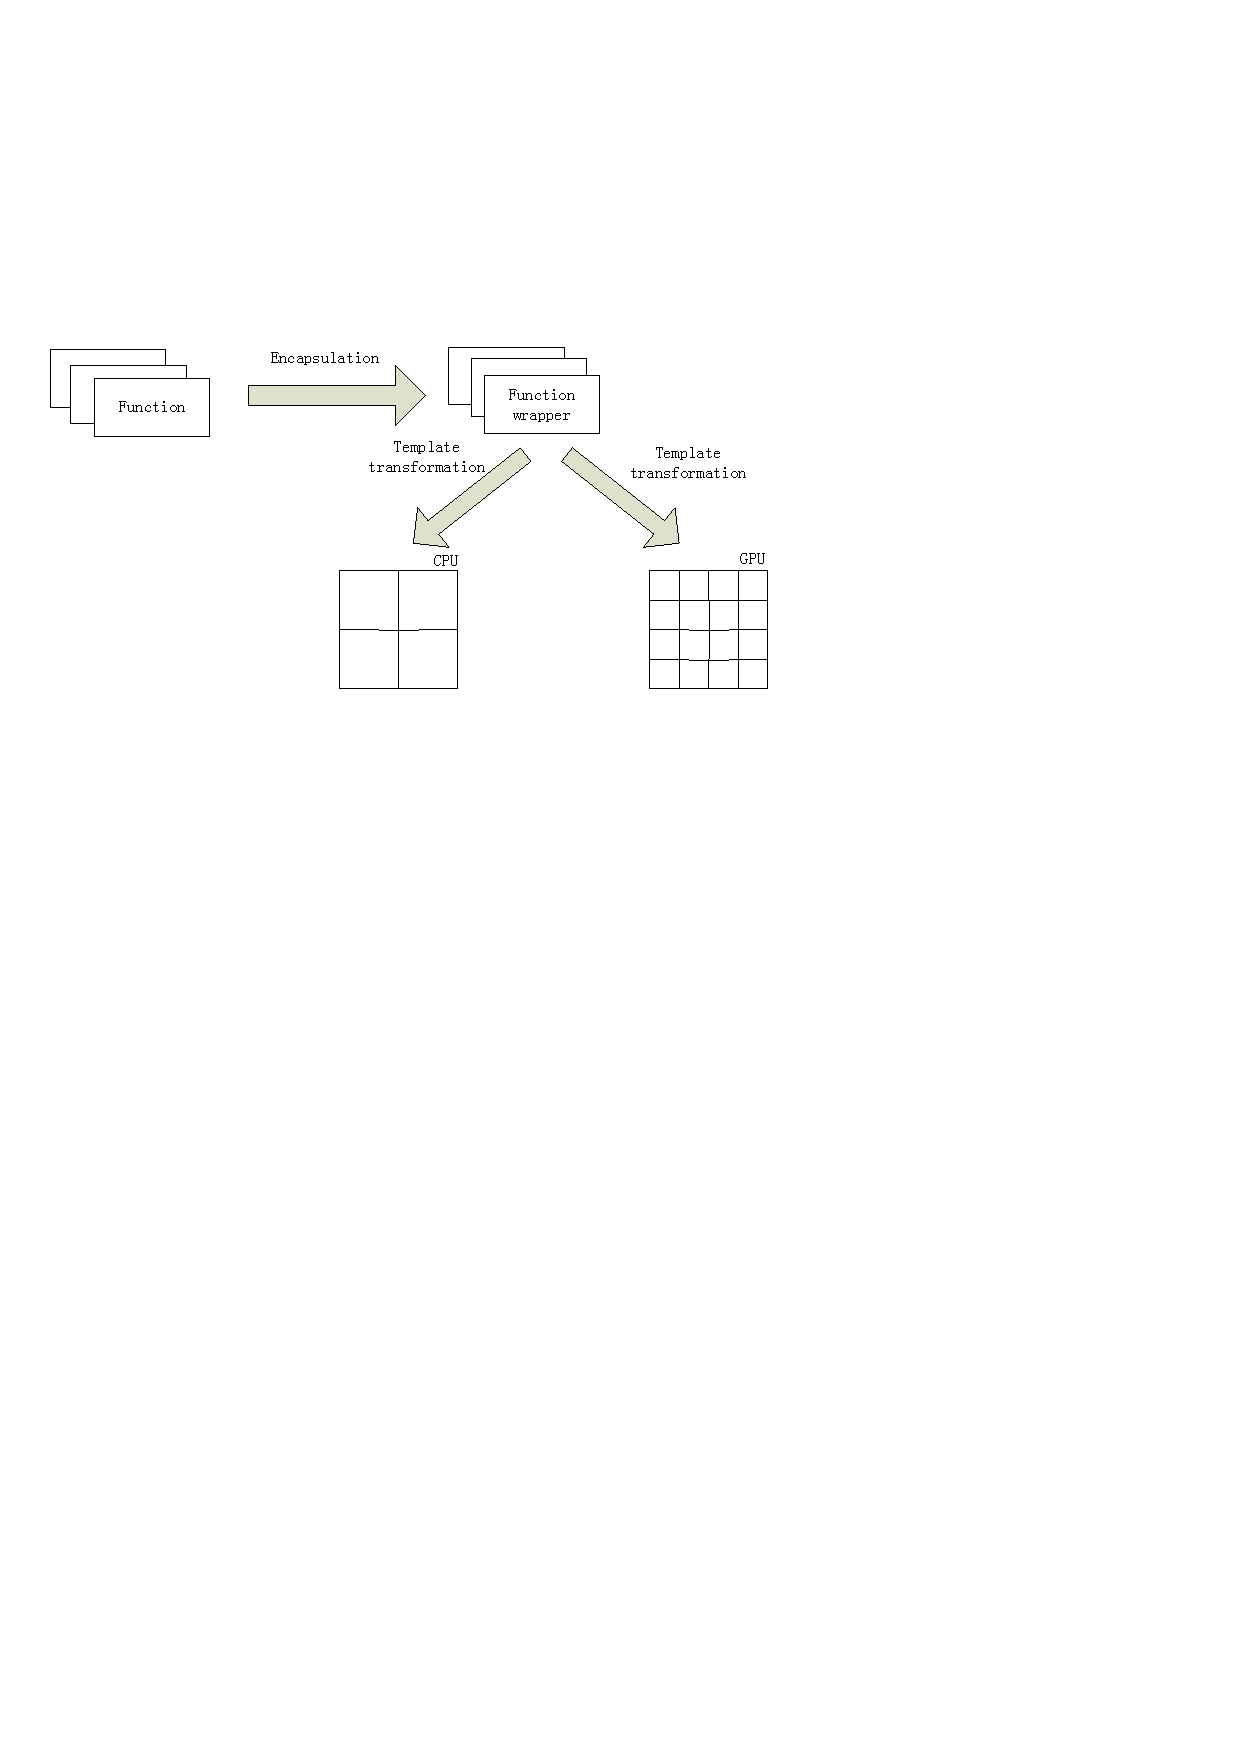
\includegraphics[width=3.3in]{../overview}
\caption{template transformation}\label{fig:overview}
\end{figure}
%programming model
Libvina framework utilizes C++ template mechanism to
perform source-to-source transformation for multicores. We uses
\emph{tasks} to abstract side-effect free functions. A task is
wrapped in the form of template class. \emph{TF classes} are able to
manipulate tasks, which take responsiblilty for transforming a tasks
into a group of subtasks. Finally, we map subtasks
into threads for specific architectures. Fig.~\ref{fig:overview}
depicts the diagram of template-based programming model.

Applications using our template-based programming model are free to
choose parallel pattern. An example using map/reduce model is shown in
Fig~\ref{fig:mmexample}. A matrix-multiplication application can be divided
into many submatrices multiplication and reduced them into the
result. We can apply a TF class dedicated to this parallel pattern and
it hierarchically generates a subtasks and reductions. The decomposition rule
and termination of recursion is programmed in template
metaprogramming.  

Our programming model facilitates to separate two roles in software
development. Algorithm-centric programmers only concern of algorithm
in convential C/C++ form. They provides computation-intensive and
side-effect free functions in the form of task. Otherwise, system
programmers known underlying architecture are charge in developing and
applying template class to specialize tasks for the concrete
target. This separation not only solve the difficulties of writing and
tuning multicore, but also providing a uniform programming model to
develop effecient and portable parallel programs.

The primary limitation of libvina framework is that we perform
transformation using template metaprorgramming.  Only static
information, \textit{i.e.} static constant value and types in C++, is
available at compile time. In libvina framework, we utilize array
dimensions to estimate problem size and divide a task into
subtasks. Thus, our programming model orients to programs which
contains rich static information.  Fortunately, it is not uncommon
that array dimensions are determinable at compile time for embeded and
scientific programs.

%Another example depicted in ~\ref{fig:pipeexample}
%illustrates another parallel pattern in our programming model. It is
%psuedo langage translationg program using pipeline processing. Applying a TF class
%for 4 the taskscan synthesize a calling chain. 
\section{Libvina Framework Design}
Libvina framework consists of 3 components: (1) supporting data
structures. (2) Transform class (3) adaptor 
